\documentclass[../Matt_Gebert_Honours_Thesis.tex]{subfiles}

\begin{document}
% In \cref{chap:baregraphene} I will present the data and results from my measurements of the respective devices which will be placed on SiO$_2$. 

Graphene devices first need to have their transport properties measured in their pristine condition, prior to the application of thin oxides. Doing this will allow a comparison of the electrical transport properties before and after transfer, to see if there's any resulting enhancement. Here I analyse the resistance measurements taken for both graphene and CVD graphene. I will consider their dependence upon gate voltage and temperature.

\section{Resistance to resistivity}
The resistivity of a material is a core property that tells you it's behaviour in a bulk geometry. For 3D materials, resistivity is in the units of Ohms per meter. You can think about this single length proportionality coming from flowing charge through a cross section, but over some length. In 2D materials, resistivity is measured in Ohms, because there are only two dimensions, the length and the width of flat material. The partial form of the resistivity is listed in \cref{eqn:partial_resistivtiy}, where $w(L)$ is the width of the material as a function of Length.\\
\begin{minipage}{0.5\textwidth}
	\begin{align}
	\partial R = \frac{\rho}{w(L)}\partial L\label{eqn:partial_resistivtiy}
	\end{align}
	In most cases of devices we make, the geometry between probes can be described by either a rectangle or a trapezoid. There will be a resulting geometric factor that converts our resistance to resistivity.
	\begin{align}
	\rho = \mathcal{G} \times R
	\end{align}
\end{minipage}
\begin{minipage}{0.5\textwidth}
%	\begin{figure}
	\centering
	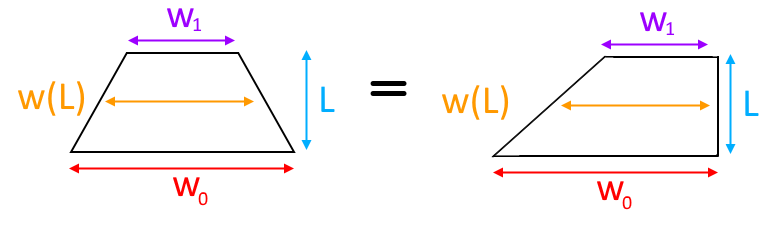
\includegraphics[width=0.9\textwidth]{chap4/geometry}
	\captionof{figure}{Two equivalent geometries of trapezoids.}
%	\end{figure}
\end{minipage}\\

For a rectangle, the width is independent of the length, and the geometric factor to convert resistance to resistivity becomes:
\begin{align}
\mathcal{G} = \frac{w}{L}
\end{align}
For a trapezoid, such as in  the width is linearly dependent upon length, and the geometric factor can be found as follows:
\begin{align}
	w(x) &= w_0 + \frac{x}{L}(w_1 - w_0)\\
	\frac{1}{\mathcal{G}} &= \int_{0}^{L}\frac{1}{w(x)}dx = \frac{l \left(\log\left[l w_0\right] - \log\left[l w_1\right]\right)}{w_0-w_1} = \frac{l \log\left[w_0/w_1\right]}{w_0-w_1}\\
	\implies \mathcal{G} &= \frac{w_0-w_1}{l \log\left[w_0 / w_1\right]}
\end{align}
In the limit w$_1\to$w$_2$, this result is consistent and returns to the rectangular case.

This quantity is ill defined for the transferred CVD graphene on top of gold pads, however the relevant geometric quantity can still be found through the gate voltage dependent resistivity (Refer to \cref{sec:findinggeometricfactor}).



\section{Gate dependent conductivity}

\subsection{Finding the geometric factor of CVD graphene}\label{sec:findinggeometricfactor}


\section{Exfoliated}\label{sec:pristine_exfoliated}



\section{CVD}\label{sec:pristine_cvd}

\begin{align}
	C_{\text{flake}} = \frac{G_{\text{SiO}_2}-G_{\text{flake}}}{G_{\text{SiO}_2}}
\end{align}

\begin{align}
	\pd R = \frac{\rho}{w} \pd L
\end{align}

\begin{align}
	R = \frac{V}{I} = \frac{V_a-V_b}{I_{in}}
\end{align}

\begin{align}
	\sigma = \sqrt{\left(N^* e \mu\right)^2 + \left(\rho_S + \frac{1}{N e \mu}\right)^{-2}}\\
	N = \frac{C_g}{e} \left|V-V_G\right|
\end{align}

\begin{align}
	\rho[V_g,T] = \rho_0[V_g] + \rho_A[T] + \rho_B[Vg,T]
\end{align}

\begin{align}
	\rho_A[T] = \left(\frac{h}{e^2}\right) \frac{\pi2 Da^2 k_B T}{2 h^2 \rho_S V_s^2 V_F^2}
\end{align}

\begin{align}
\rho_B[V_G,T]&= B \frac{h}{e^2} V_G^{-\alpha_1} \left(\begin{aligned}
&\frac{1}{\exp\left[(0.059\text{ eV})/k_B T\right]-1}\\ &\hspace{2cm}+\frac{6.5}{\exp\left[(0.115\text{ eV})/k_B T\right]-1}
\end{aligned}\right)
\end{align}

\subsection{hBN transfer}


\end{document}